\documentclass[12pt,a4paper]{article}

\usepackage[utf8]{inputenc}
\usepackage[latvian]{babel}
\usepackage{caption}

\usepackage{hyperref}

% Make captions "1. attēls."
\DeclareCaptionLabelFormat{numberfirst}{\arabic{figure}. attēls}
\captionsetup[figure]{labelformat=numberfirst,labelsep=period}

% Command for referencing: "1. attēls"
\newcommand{\figref}[1]{\ref{#1} attēls}


\pagenumbering{arabic} % Sets page numbering to arabic (1, 2, 3, ...)
\setcounter{page}{1} % Specifies the starting page number

\usepackage{tabularx} % in your preamble
\usepackage{amsmath, amssymb}
\usepackage{graphicx}
\usepackage{geometry}
\usepackage{subcaption}
\usepackage{float}
\usepackage{array}
\usepackage{booktabs}
\usepackage{enumitem}
\usepackage{fancyhdr}
\usepackage{xcolor}
\usepackage{framed}
\usepackage{titlesec}

% Example 1: Bold, larger font, with some vertical spacing
\titleformat{\section}
  {\normalfont\Large\bfseries} % format: font + weight
  {\thesection}                % label (number)
  {0.3em}                         % space between number and title
  {}                            % code before title text

\geometry{
    left=2cm,
    right=2cm,
    top=2.5cm,
    bottom=2.5cm
}

\pagestyle{plain}
\fancyhf{}
\rhead{Orbitāles un ķīmiskās saites}

% Custom colors and environments
\definecolor{taskbg}{rgb}{0.95,0.95,0.95}

% Custom environment for tasks
\newenvironment{taskbox}
{\begin{framed}\begin{minipage}{\textwidth}}
{\end{minipage}\end{framed}}

\title{\textbf{Orbitāles un ķīmiskās saites}}
\author{}
\date{}

\begin{document}

\maketitle

\section{Atomu orbitāles}

Elementa kārtas skaitlis apzīmē tā protonu un elektronu skaitu, piemēram, oglekļa atomu veido 6 protoni un 6 elektroni. Atoma kodols aizņem tikai $10^{-12}$ daļu no atoma telpas, pārējo daļu aizņem kustībā esoši elektroni. Tie ir izkliedēti pa visu atoma telpu, taču atkarībā no to enerģijas, elektronu atrašanās sadalījums mainās. \textbf{Orbitāle} ir tā atoma telpas daļa, kurā noteikti atrodas elektrons. Orbitāles tiek attēlotas kā virsmas, kas ietver elektronu ar varbūtību 0.9 (\figref{fig:orbitales}).

\begin{figure}[H]
    \centering
    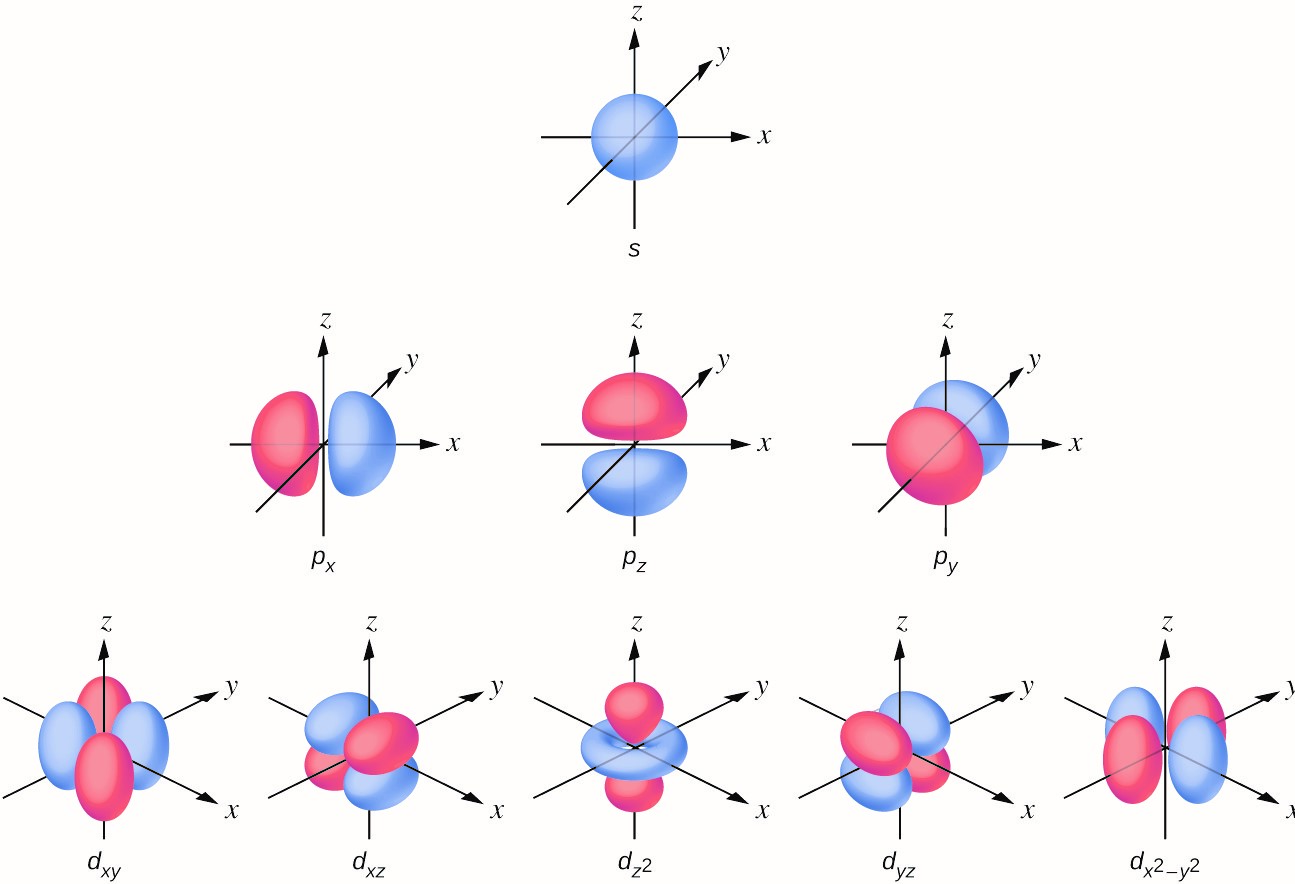
\includegraphics[width=0.5\textwidth]{atteli/orbitales.jpg}
    \caption{Orbitāļu attēlojums.}
    \label{fig:orbitales}
\end{figure}

Elektronu enerģijas vērtības apzīmē ar \textbf{līmeņiem} (1, 2, 3, ...) un \textbf{apakšlīmeņiem} (\textit{s}, \textit{p}, \textit{d}, \textit{f}). Elektronu un tā orbitāli attiecīgi apakšlīmenim dēvē par \textit{s}, \textit{p}, \textit{d}, \textit{f} elektronu vai orbitāli.

\begin{itemize}
    \item Katrā enerģijas līmenī ir viena \textit{s} orbitāle.
    \item Sākot ar otro enerģijas līmeni pievienojas trīs \textit{p} orbitāles.
    \item Sākot ar trešo enerģijas līmeni pievienojas piecas \textit{d} orbitāles.
\end{itemize}

Orbitālē var atrasties elektronu pāris vai viens nepārots elektrons. Sapāroties var elektroni ar pretējiem spiniem, ko apzīmē ar $\uparrow \downarrow$. Orbitāļu shēmu zīmēšana parādīta \ref{fig:konfiguracijas} attēlā. Elektroni vispirms novietojas brīvā orbitālē ar zemāko enerģiju, ja nav brīva cita tās pašas enerģijas orbitāle, tad tas sapārojas ar citu elektronu šajā orbitālē. Orbitāļu aizpildīšanās secība parādīta \ref{fig:steps} attēlā.

\begin{figure}[H]
    \centering
    \begin{subfigure}[b]{0.49\textwidth}
        \centering
        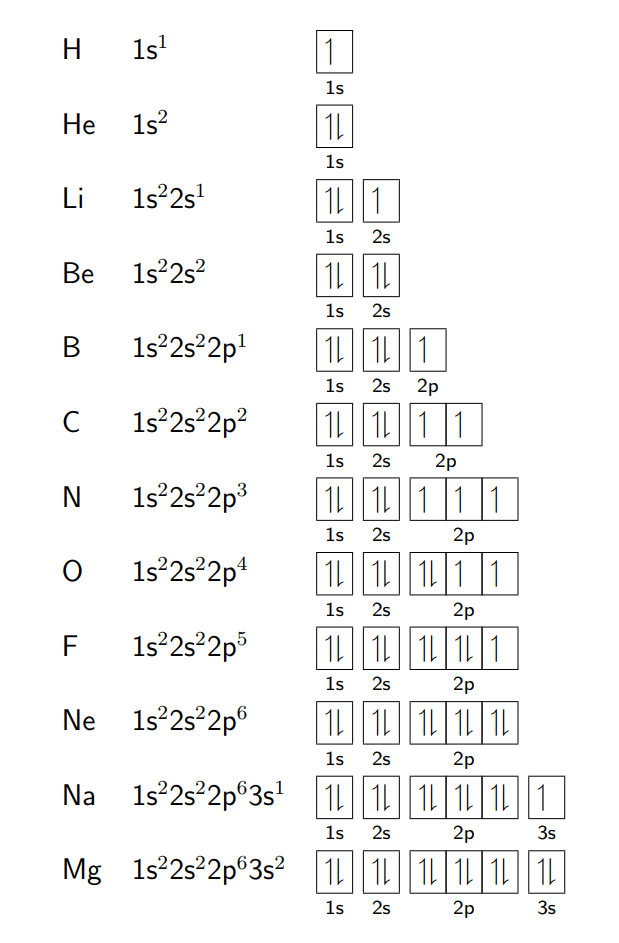
\includegraphics[width=0.7\textwidth]{atteli/konfiguracijas.png}
        \caption{Elektronformulas un orbitāļu diagrammas atomiem līdz 3\textit{s} orbitālei.}
        \label{fig:konfiguracijas}
    \end{subfigure}
    \hfill
    \begin{subfigure}[b]{0.49\textwidth}
        \centering
        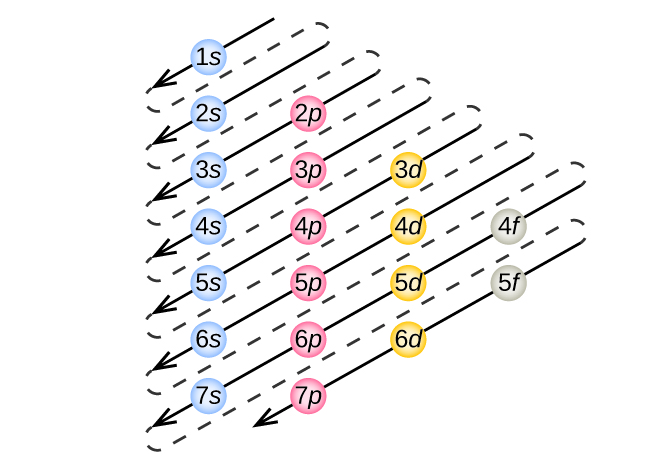
\includegraphics[width=\textwidth]{atteli/steps.jpg}
        \caption{Elektronu pildīšanās secība apakšlīmeņos.}
        \label{fig:steps}
    \end{subfigure}
    \caption{Elektronu konfigurācijas un aizpildīšanas secība.}
\end{figure}


\textbf{1. uzdevums.} Uzzīmē hlora atoma orbitāļu diagrammu kā attēlā \ref{fig:konfiguracijas} un nosaki \\ elektronformulu!

Ķīmisku saiti veido elektronu pāris, kurš atrodas orbitālē, kuru dēvē par molekulāru orbitāli (MO). Šie elektroni var atrasties gan viena, gan otra atoma telpā, un ķīmiskās saites iedala pēc šī sadalījuma.

\begin{table}[H]
\centering
\begin{tabularx}{\textwidth}{|
    >{\raggedright\arraybackslash}p{4.5cm}|
    >{\raggedright\arraybackslash}X|
    >{\raggedright\arraybackslash}p{3cm}|}
\hline
\textbf{Saites veids} & \textbf{Apraksts} & \textbf{Piemēri} \\
\hline
Nepolāra kovalenta saite & Elektronu pāris pieder tikpat daudz vienam cik otram atomam. & H$_2$, O$_2$, N$_2$ \\
\hline
Polāra kovalenta saite & Ap viena atoma elektronu atrašanās varbūtība ir lielāka. Šim atomam ir daļēji negatīvs lādiņš, bet otram tikpat daļēji pozitīvs. & HCl, H$_2$S, NH$_3$ \\
\hline
Jonu saite & Elektronu pāris atrodas gandrīz tikai viena atoma telpā. Atomi pārvēršas par joniem un turas kopā elektrostatiski. & NaCl, KBr, Na$_2$S \\
\hline
\end{tabularx}
\end{table}


\section{Luisa struktūras}

Luisa simbolu veido elementa simbols un punkti, kuri apzīmē šī elementa ārējā līmeņa jeb valences elektronus. Valences elektronu skaitu A grupas elementiem var noteikt pēc to grupas numura (skat. \ref{fig:luisa_simboli} attēlu ).

\begin{figure}[H]
    \centering
    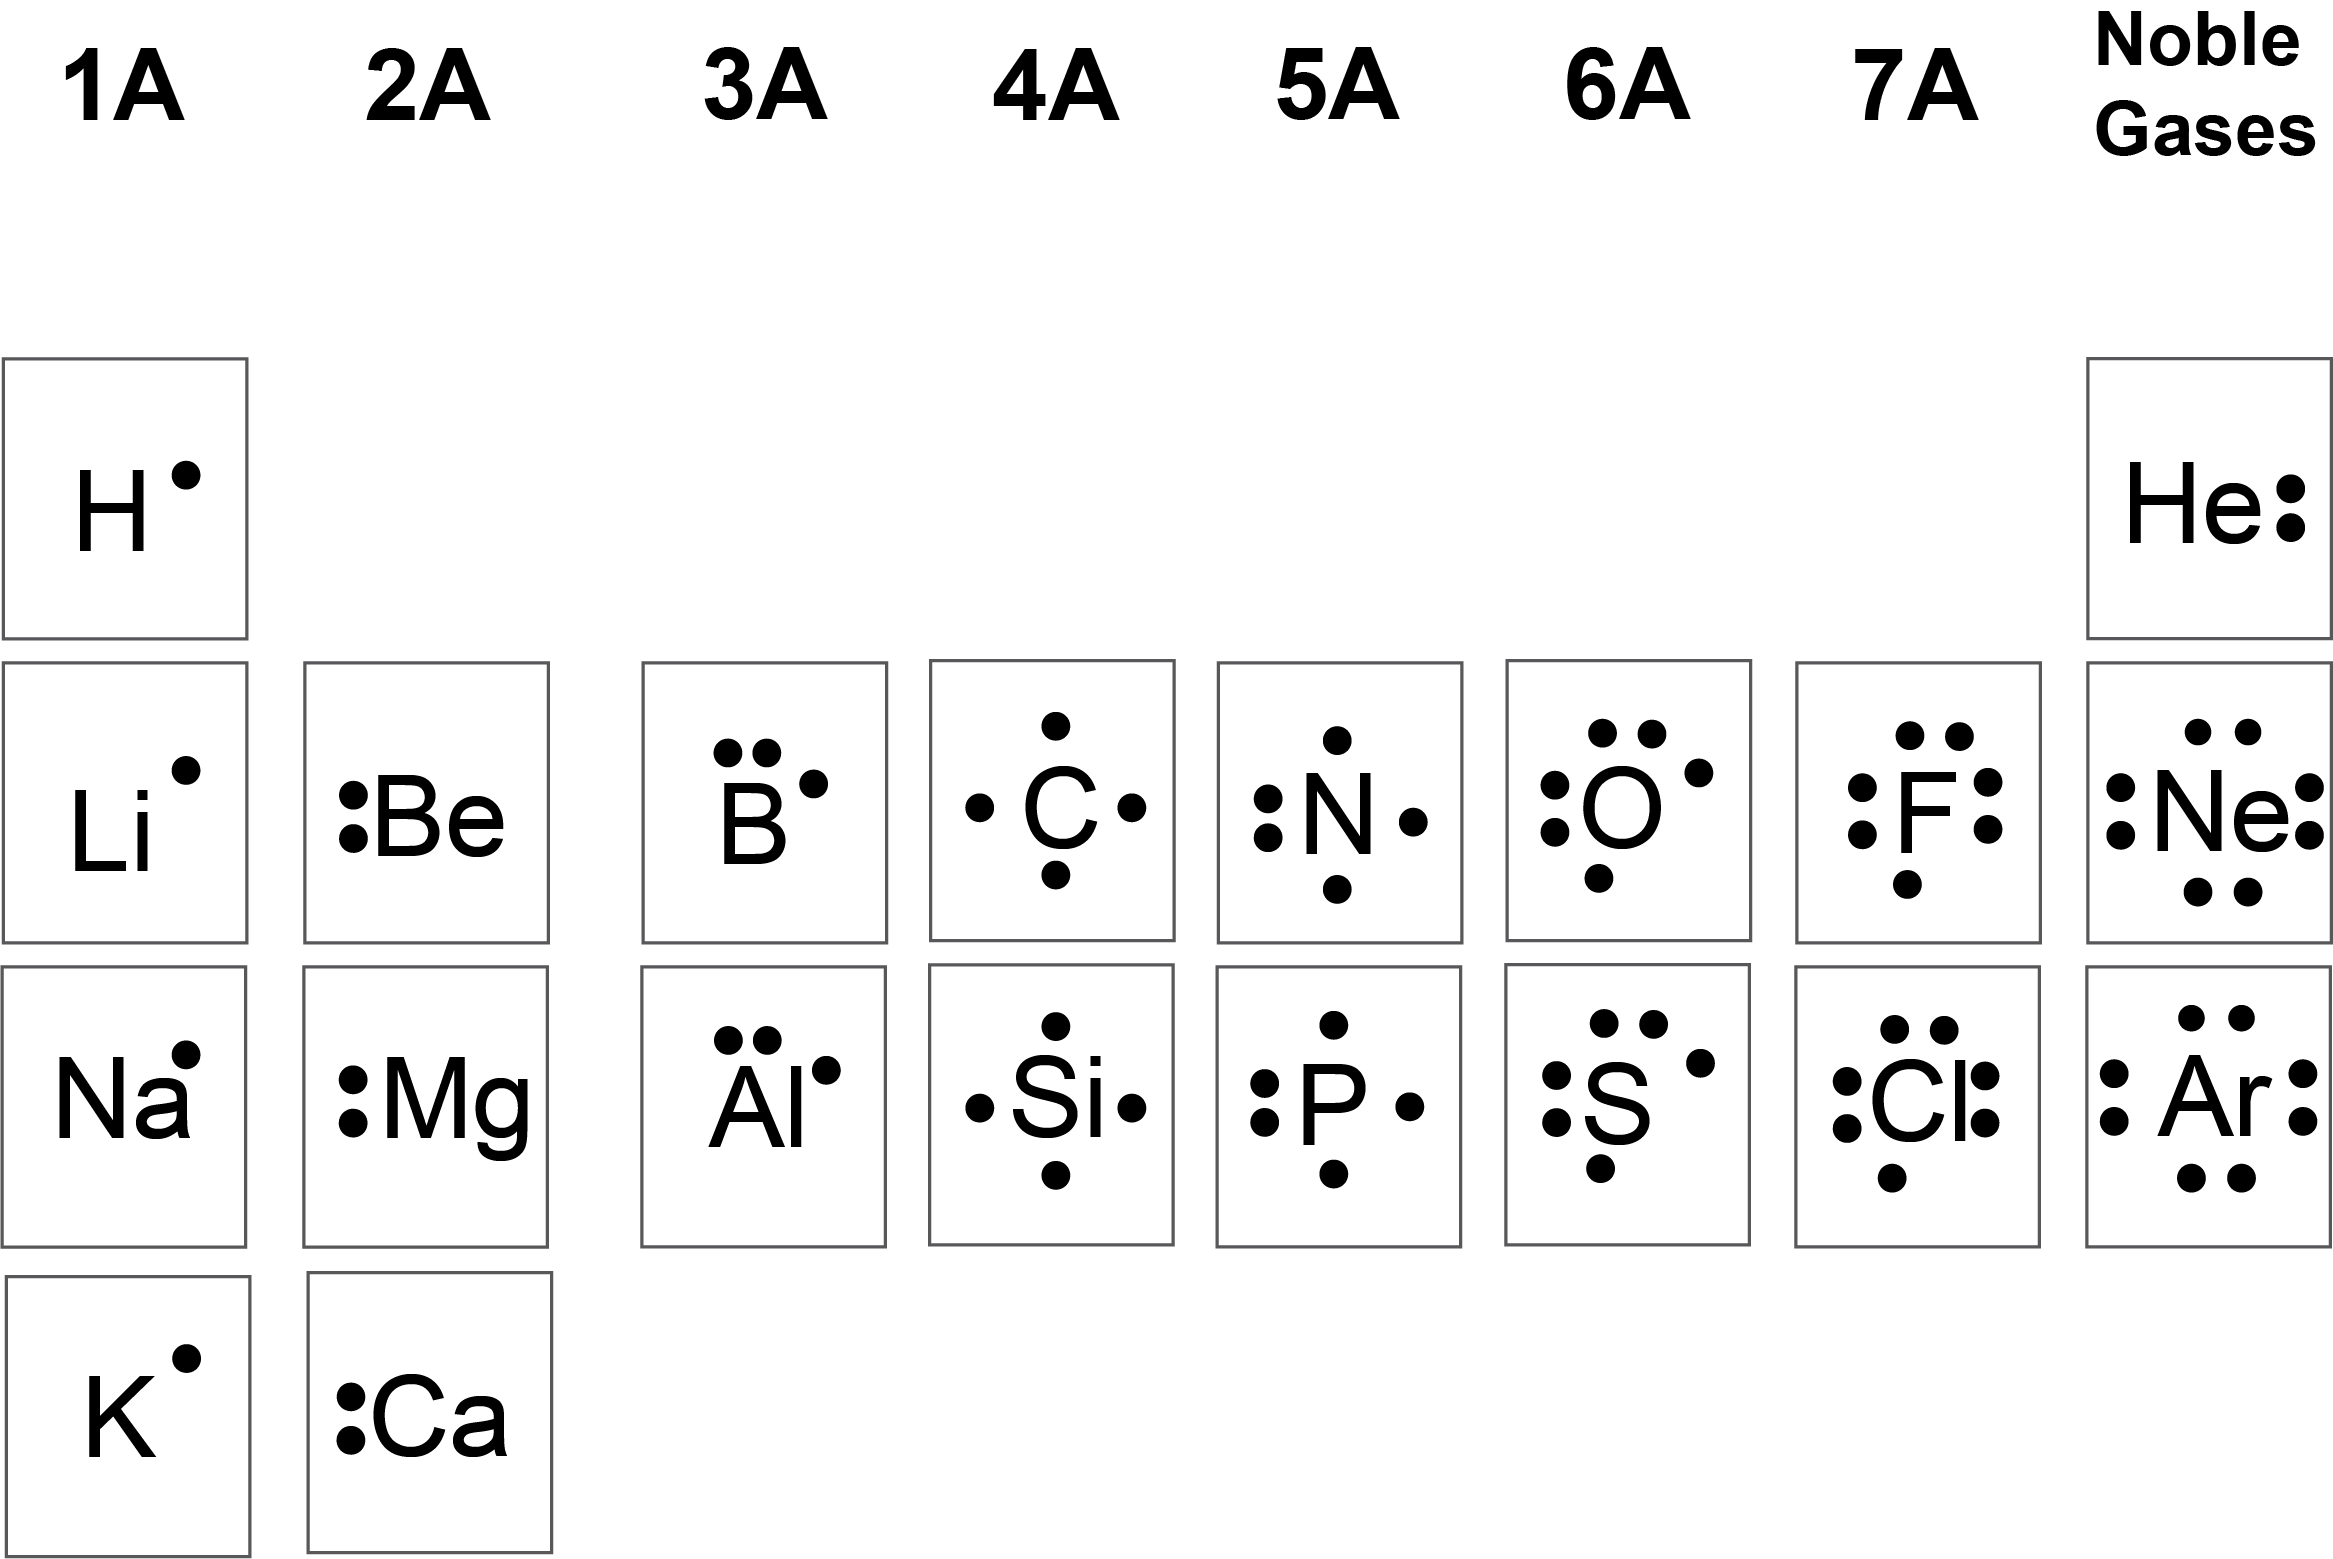
\includegraphics[width=0.5\textwidth]{atteli/Luisa_simboli.png}
    \caption{Luisa simboli A grupu elementiem.}
    \label{fig:luisa_simboli}
\end{figure}

Ar Luisa simboliem var parādīt kovalento saišu veidošanos. \textbf{Luisa struktūras} ir molekulu attēlojumi, piemēram, Cl$_2$ molekulai (skat. \ref{fig:cl_bonding} attēlu), kuri izceļ to, ka ķīmisko saiti veido elektronu pāris. Ierastāk elektronu pāri apzīmē ar svītru (skat. \ref{fig:luisa_saite} attēlu).

\begin{figure}[H]
    \centering
    \begin{subfigure}[b]{0.45\textwidth}
        \centering
        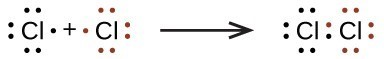
\includegraphics[width=0.7\textwidth]{atteli/Cl_bonding_edited.jpg}
        \caption{Cl$_2$ molekulas Luisa struktūra.}
        \label{fig:cl_bonding}
    \end{subfigure}
    \hfill
    \begin{subfigure}[b]{0.45\textwidth}
        \centering
        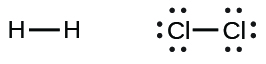
\includegraphics[width=0.6\textwidth]{atteli/Luisa_saite.jpg}
        \caption{Luisa saites attēlojums.}
        \label{fig:luisa_saite}
    \end{subfigure}
    \caption{Luisa struktūru attēlojumi.}
\end{figure}

Elementu atomiem atšķiras valences elektronu skaits, bet to, kā tie veido saites vieno \textbf{okteta likums} --- atomi dalās ar elektroniem tā, lai to ārējā enerģijas līmenī būtu astoņi elektroni. Izņēmumi ir H, He, Li un Be. Tiem kopumā ir maz elektronu, tāpēc astoņi valences elektroni tos nepadarītu stabilākus, tā vietā tie vēlas divus. Cik elektronu pietrūkst atomam lai izpildītu okteta likumu, tik kovalentās saites tas parasti veido.

Veidojoties dubultajām vai trīskāršajām saitēm, atomi savā starpā dala attiecīgi divus vai trīs elektronu pārus (\figref{fig:dubultsaite}).

\begin{figure}[H]
    \centering
    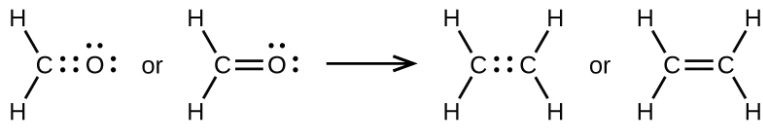
\includegraphics[width=0.5\textwidth]{atteli/dubultsaite.jpg}
    \caption{Luisa struktūras ar dubultsaiti.}
    \label{fig:dubultsaite}
\end{figure}

\begin{taskbox}
\textbf{2. uzdevums.}
Cik kovalentās saites veido O, N un C atoms?
\end{taskbox}

\section{Molekulāro orbitāļu teorija}

Līdz šim mēs ķīmisko saiti definējām kā elektronu pāri. Tagad aplūkosim, kā dažādos veidos elektronu orbitāles savā starpā mijiedarbojoties veido molekulārās orbitāles (MO), kas ir pamatā ķīmiskajai saitei.

Pārklājoties divām \textit{s} orbitālēm, piemēram diviem H atomiem, veidojas $\sigma$ molekulārā orbitāle. Elektroniem ir gan daļiņu, gan viļņu raksturs, tāpēc, ja abu elektronu viļņi ir vienā fāzē, veidojas zemas enerģijas $\sigma_s$ MO, savukārt, ja elektronu viļņi ir pretfāzē, veidojas augstas enerģijas nesaistošā $\sigma_s^*$ MO (\figref{fig:sigma}). Tikai no zemas enerģijas MO veidojas ķīmiskā saite.

Turklāt $\sigma$ saites var veidoties arī no pretēji novietotām \textit{p} orbitālēm, kuras pārklājas (\figref{fig:p_sigma}).

\begin{figure}[H]
    \centering
    \begin{subfigure}[b]{0.45\textwidth}
        \centering
        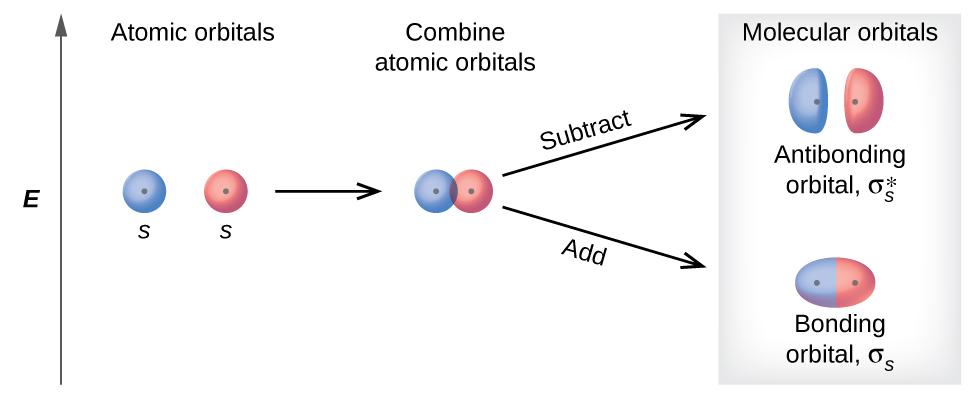
\includegraphics[width=\textwidth]{atteli/sigma.jpg}
        \caption{$\sigma$ molekulāro orbitāļu veidošanās no \textit{s} orbitālēm.}
        \label{fig:sigma}
    \end{subfigure}
    \hfill
    \begin{subfigure}[b]{0.45\textwidth}
        \centering
        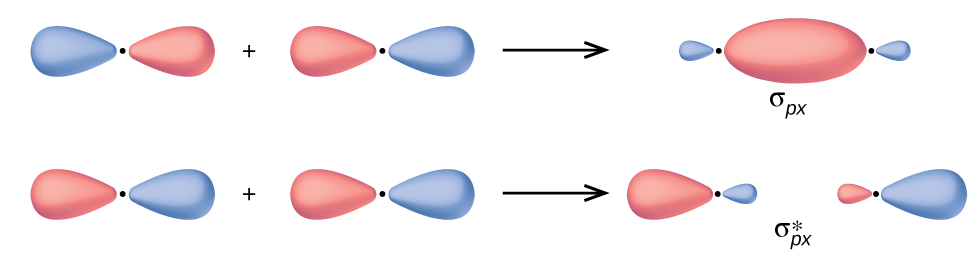
\includegraphics[width=\textwidth]{atteli/p_sigma.jpg}
        \caption{$\sigma$ molekulāro orbitāļu veidošānās no \textit{p} orbitālēm. Ar krāsām apzīmē elektronu viļņu fāzes.}
        \label{fig:p_sigma}
    \end{subfigure}
    \caption{$\sigma$ molekulāro orbitāļu veidošanās.}
\end{figure}

Sāniski pārklājoties \textit{p} orbitāles veido $\pi$ molekulārās orbitāles (\figref{fig:p_pi}).

\begin{figure}[H]
    \centering
    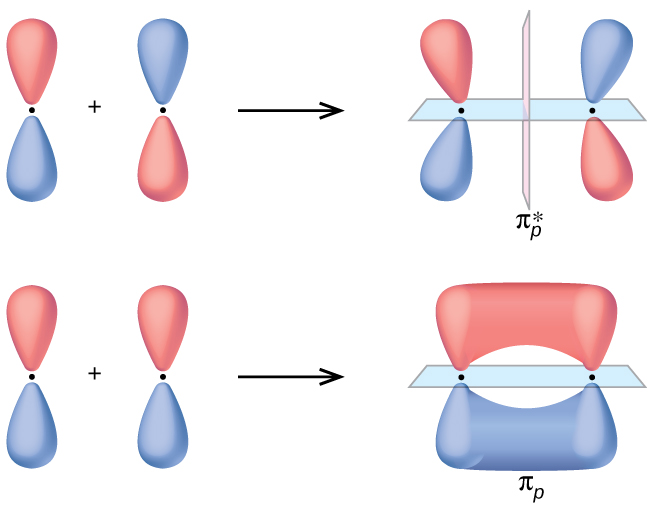
\includegraphics[width=0.3\textwidth]{atteli/p_pi.jpg}
    \caption{$\pi$ molekulāro orbitāļu veidošanās no \textit{p} orbitālēm.}
    \label{fig:p_pi}
\end{figure}

Pēdējais knifs, ko aplūkosim ir saišu hibridizācija. Ja aplūkoji C atoma elektronu konfigurāciju 2. attēlā, varbūt ievēroji, ka, lai aizpildītos pēdējā \textit{p} orbitāle, C atomam būtu jāiegūst vesels elektronu pāris no cita atoma. Lietas notiek citādi. Vienā no gadījumiem 2\textit{s} orbitāle hibridizējas ar trīs 2\textit{p} orbitālēm, veidojot četras \textit{sp}$^3$ orbitāles. Šīs orbitāles var veidot $\sigma$ saites, piemēram ar H vai C atomiem, veidojot alkānus (\figref{fig:ethane}).

\begin{figure}[H]
    \centering
    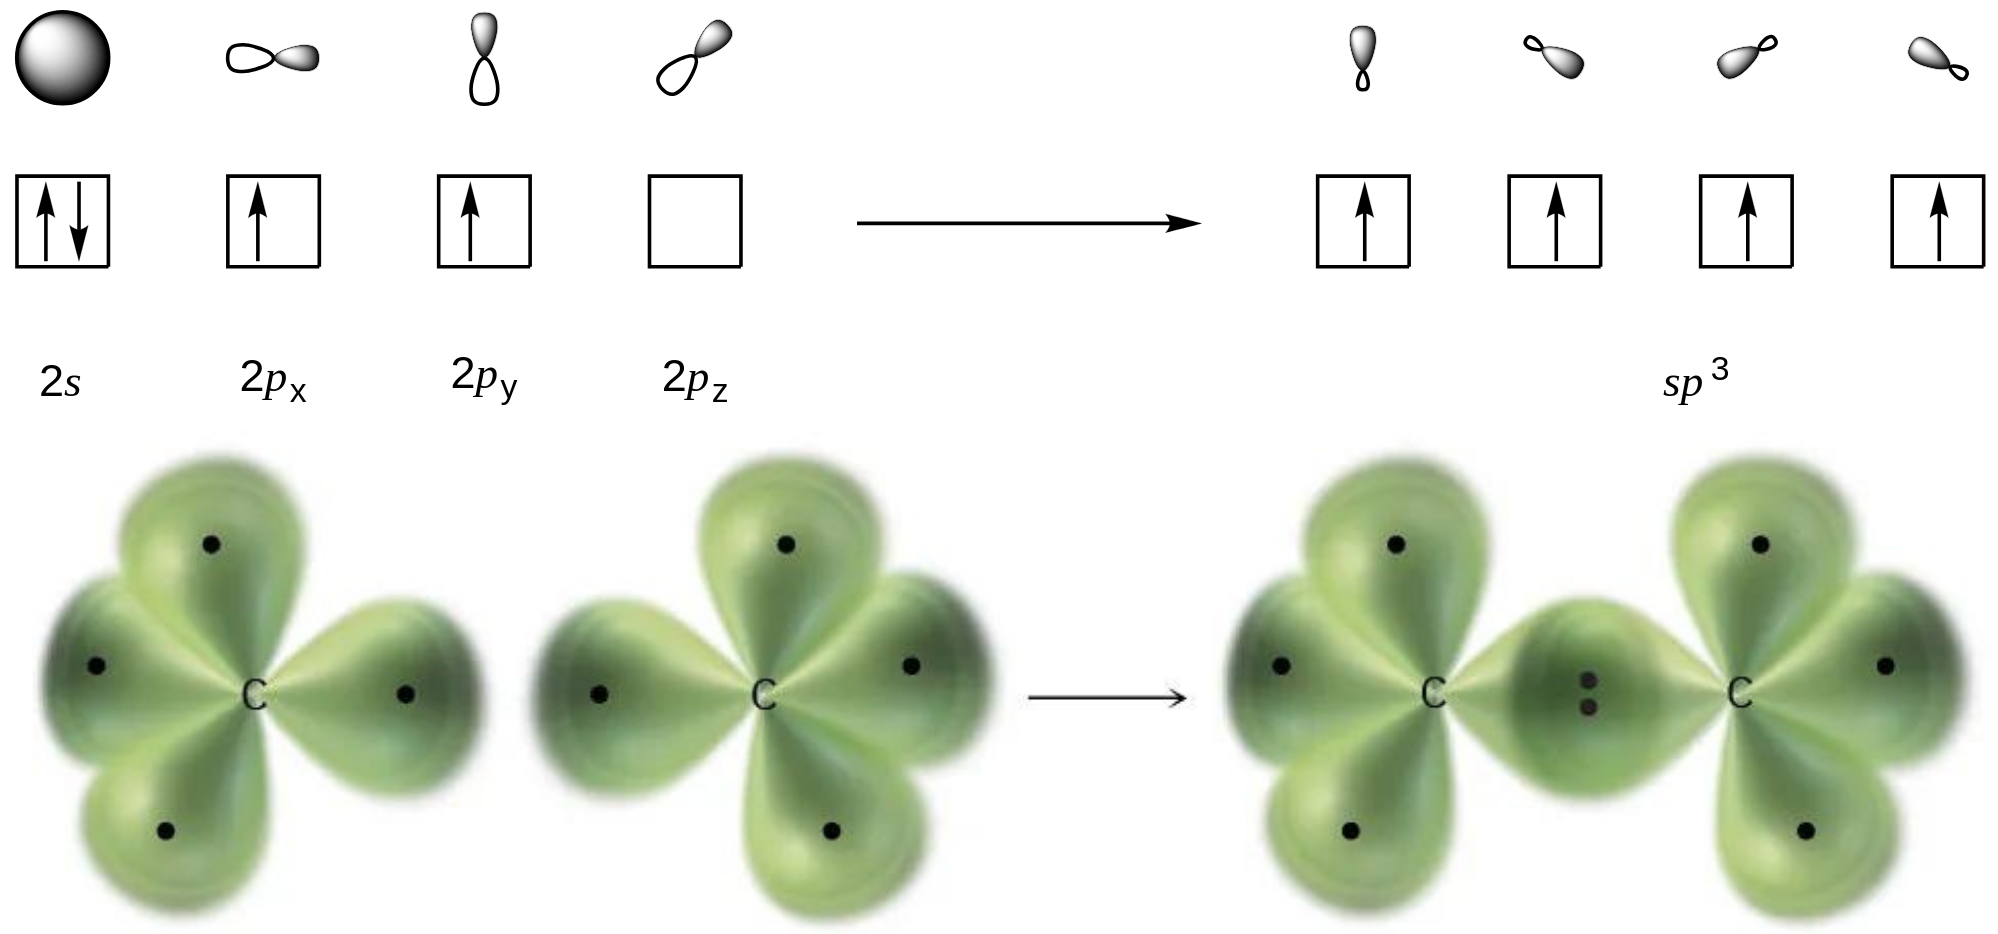
\includegraphics[width=0.5\textwidth]{atteli/ethane.png}
    \caption{\textit{sp}$^3$ hibridizācija un etāna saites.}
    \label{fig:ethane}
\end{figure}

Tāpat 2\textit{s} orbitāle var hibridizēties ar divām vai vienu 2\textit{p} orbitāli, veidojot attiecīgi trīs \textit{sp}$^2$ orbitāles vai divas \textit{sp} orbitāles. Atlikusās orbitāles ir \textit{p} orbitāles, tāpēc tagad var veidoties $\sigma$ un $\pi$ saites reizē, veidojot dubultās (\figref{fig:ethylene}) vai trīskāršās saites (\figref{fig:acetylene}).

\begin{figure}[H]
    \centering
    \begin{subfigure}[b]{0.45\textwidth}
        \centering
        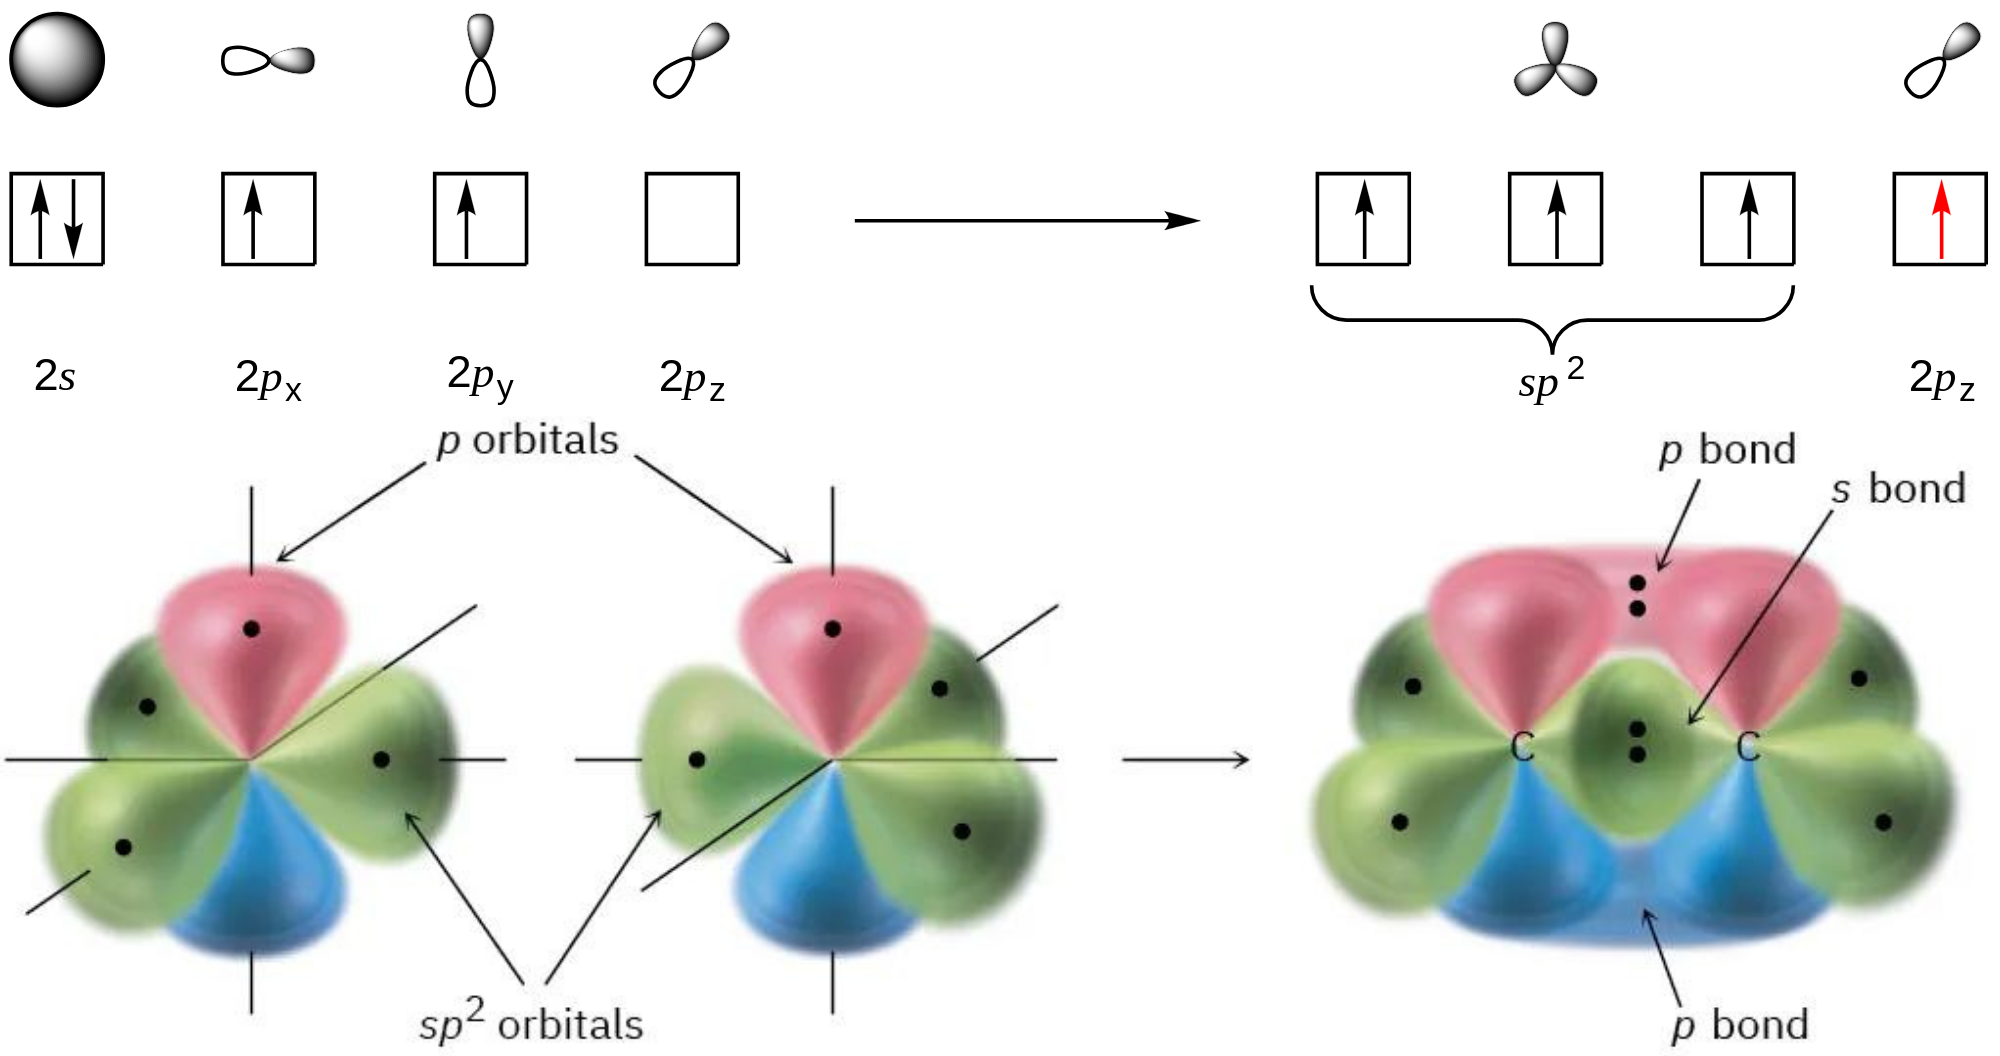
\includegraphics[width=\textwidth]{atteli/ethylene.png}
        \caption{\textit{sp}$^2$ hibridizācija un etēna saites.}
        \label{fig:ethylene}
    \end{subfigure}
    \hfill
    \begin{subfigure}[b]{0.45\textwidth}
        \centering
        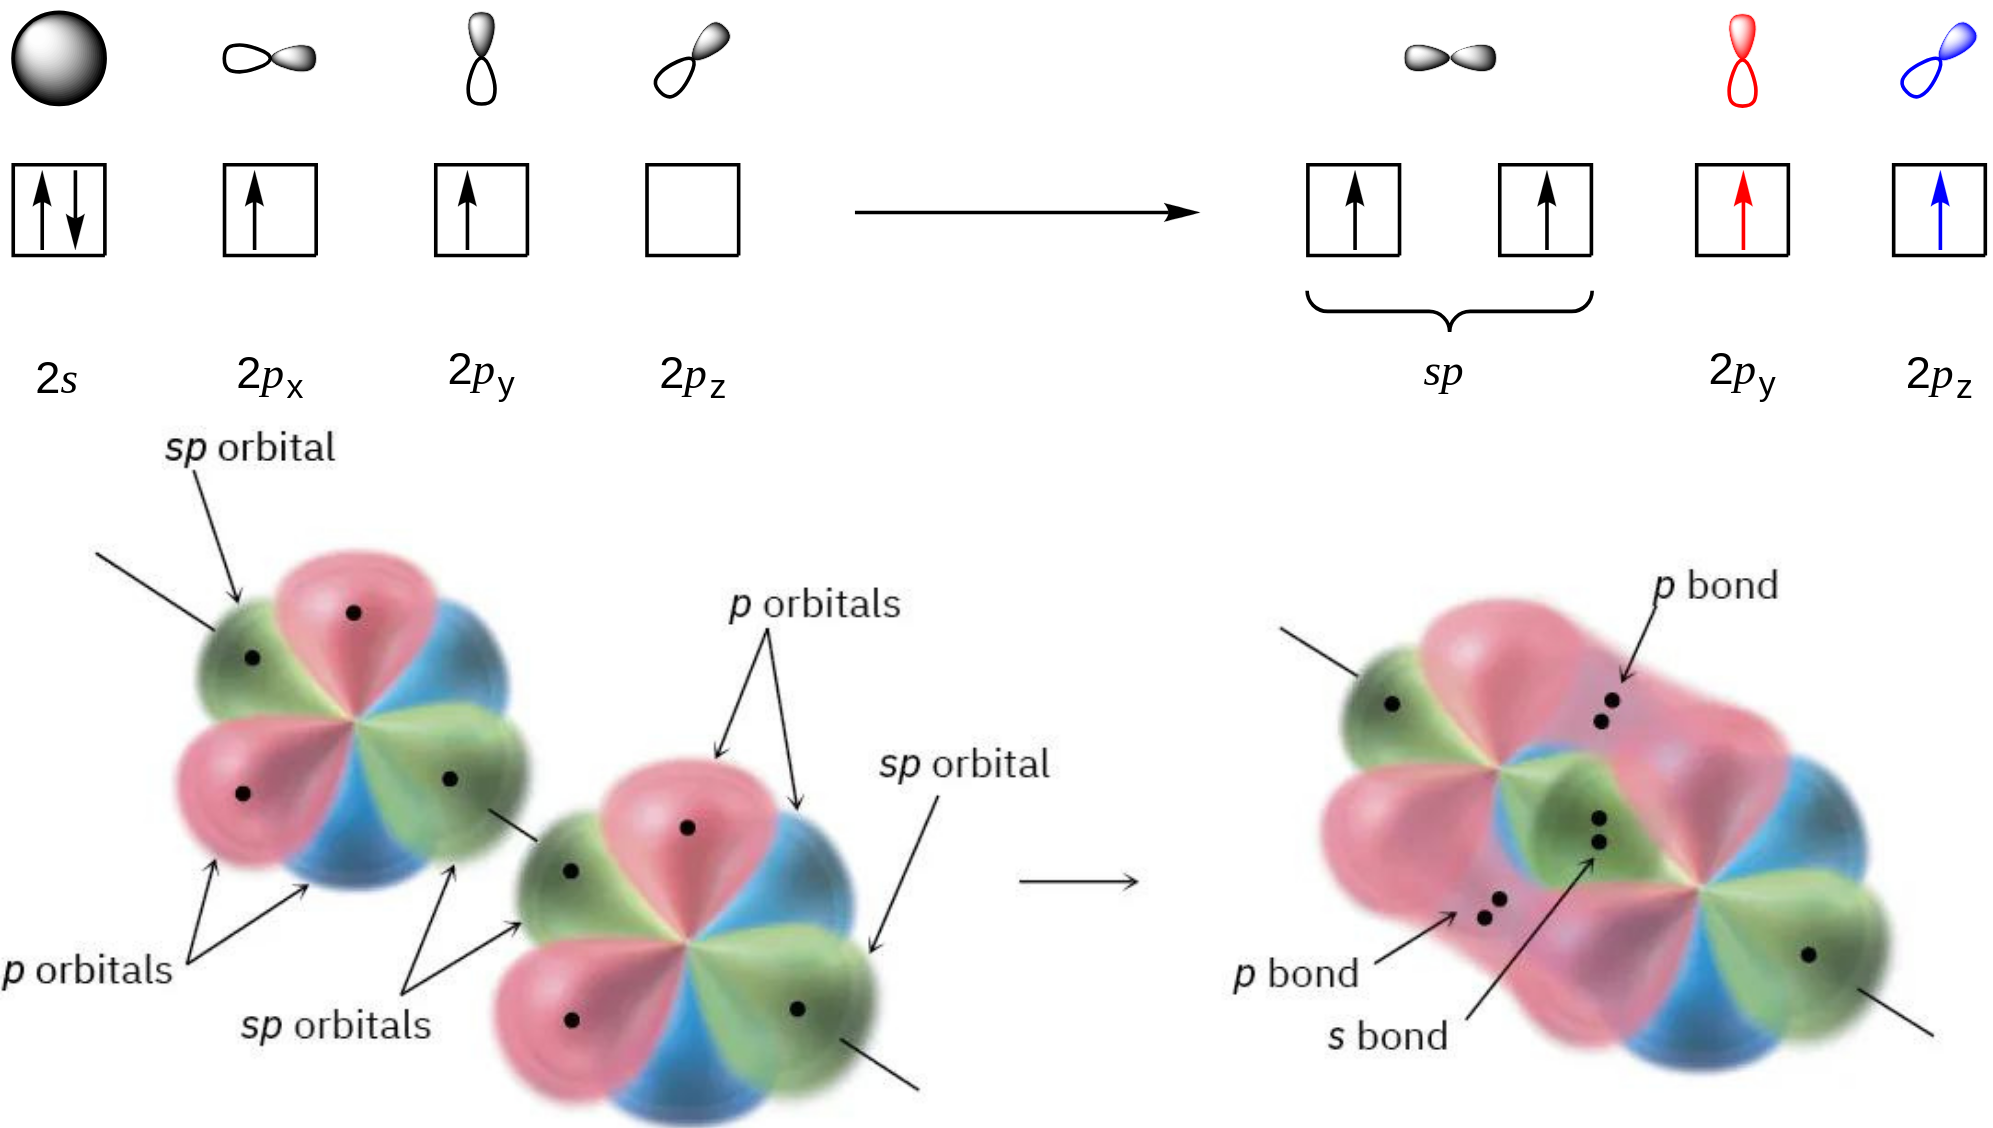
\includegraphics[width=\textwidth]{atteli/acetylene.png}
        \caption{\textit{sp} hibridizācija un etīna saites.}
        \label{fig:acetylene}
    \end{subfigure}
    \caption{Hibridizācijas veidi.}
\end{figure}

Ja ķīmiskajai saitei pievada atbilstošu enerģiju, piemēram, elektromagnētisko viļņu veidā, viens no tās elektroniem var pāriet augstas enerģijas MO, tādējādi saraujot saiti. Tā kā $\pi$ saitēs atomu orbitāles mazāk pārklājas nekā $\sigma$ saitēs, tās ir vieglāk saraut (\figref{fig:h2} un \figref{fig:pipi}).

\begin{figure}[H]
    \centering

    \begin{subfigure}[b]{0.45\textwidth}
        \centering
        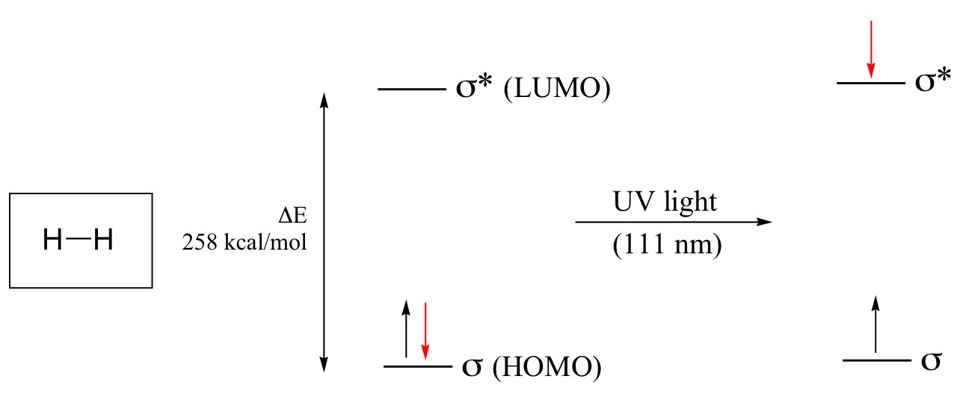
\includegraphics[width=\textwidth]{atteli/H2.jpg}
        \caption{Nepieciešamā enerģija (gaismas vilnis) $\sigma$ saites saraušanai H$_2$.}
        \label{fig:h2}
    \end{subfigure}
    \hfill
    \begin{subfigure}[b]{0.45\textwidth}
        \centering
        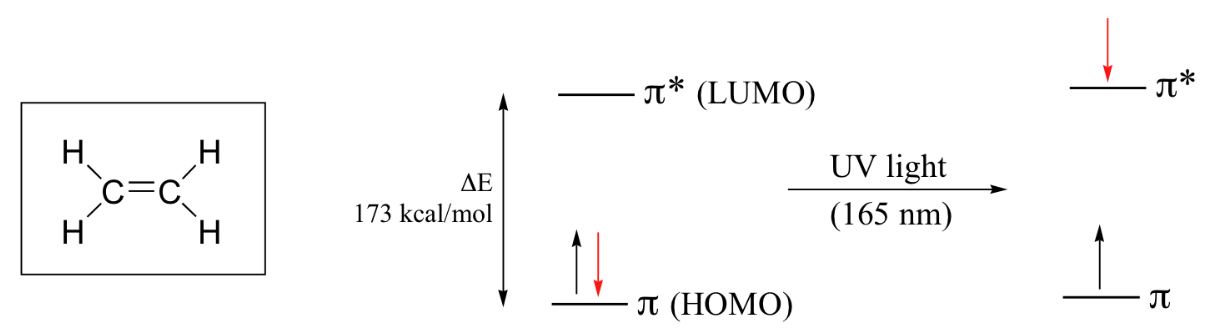
\includegraphics[width=\textwidth]{atteli/pipi.png}
        \caption{Nepieciešamā enerģija (gaismas vilnis) $\pi$ saites saraušanai C$_2$H$_4$.}
        \label{fig:pipi}
    \end{subfigure}
    \caption{Saišu saraušanas enerģijas.}
    \label{sarausana}
\end{figure}

\begin{taskbox}
\textbf{3. uzdevums.} Padomā, kāda molekulārā orbitāles veidojas (un vai tā veidojas) un \\ 
izvēlies gadījumu(s), kad veidojas ķīmiskā saite!

\makebox[\linewidth]{%
    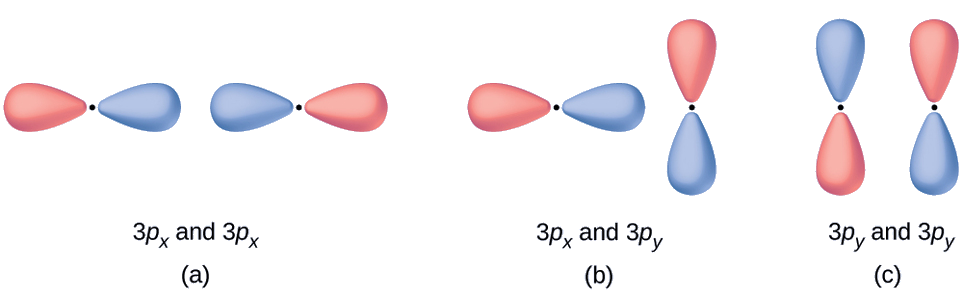
\includegraphics[width=0.7\textwidth]{atteli/task.png}%
}
\end{taskbox}



\section*{Atsauces}

Chemistry (Open Stax), Paul Flowers, Klaus Theopold, Richard Langley \& William R. Robinson, darbs ir licencēts saskaņā ar CC BY 4.0. Bezmaksas pieeja \href{https://openstax.org/books/chemistry-2e/pages/1-introduction}{Chemistry (OpenStax)}.

\newpage
\section*{Atbildes}

\textbf{1. uzdevums.}
\begin{figure}[H]
    \centering
    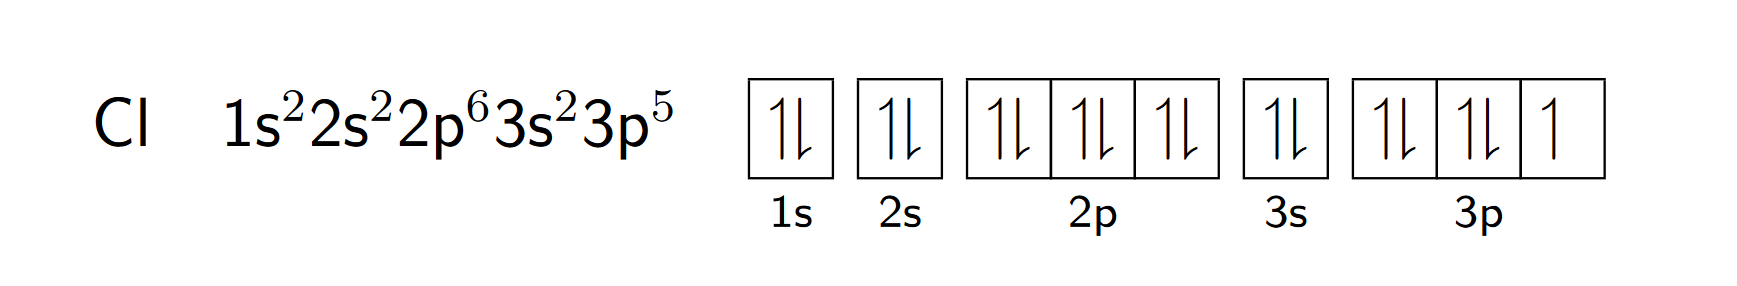
\includegraphics[width=0.7\textwidth]{atteli/Cl.png}
\end{figure}

\textbf{2. uzdevums.}
 O veido 2 saites. N veido 3 saites. C veido 4 saites.

\textbf{3. uzdevums.}
(a) gadījumā veidojas $\sigma_p$ molekulārā orbitāle un saite. (b) gadījumā orbitāles nepārklājas, neveidojas molekulārā orbitāle. (c) gadījumā veidojas $\pi_p^*$ molekulārā orbitāle, tāpēc ķīmiskā saite neveidojas.

\end{document}